% --- V-JEPA 2 (Assran et al., arXiv:2506.09985) ---
\begin{frame}{V-JEPA 2: Scaling Video JEPA for Understanding and Planning}
  \begin{columns}[T,onlytextwidth]
    \column{0.42\textwidth}
    Same \textbf{visual mask denoising} / JEPA spirit as I-JEPA, but at \textbf{internet scale}    
    \vspace{0.2em}
      \begin{itemize}
          \item Order of \textbf{$\sim$1M hours} of video and \textbf{$\sim$1M images} for pre-training.
          \item Downstream use: video understanding, video QA, and planning.
      \end{itemize}
    \column{0.56\textwidth}
      \centering
      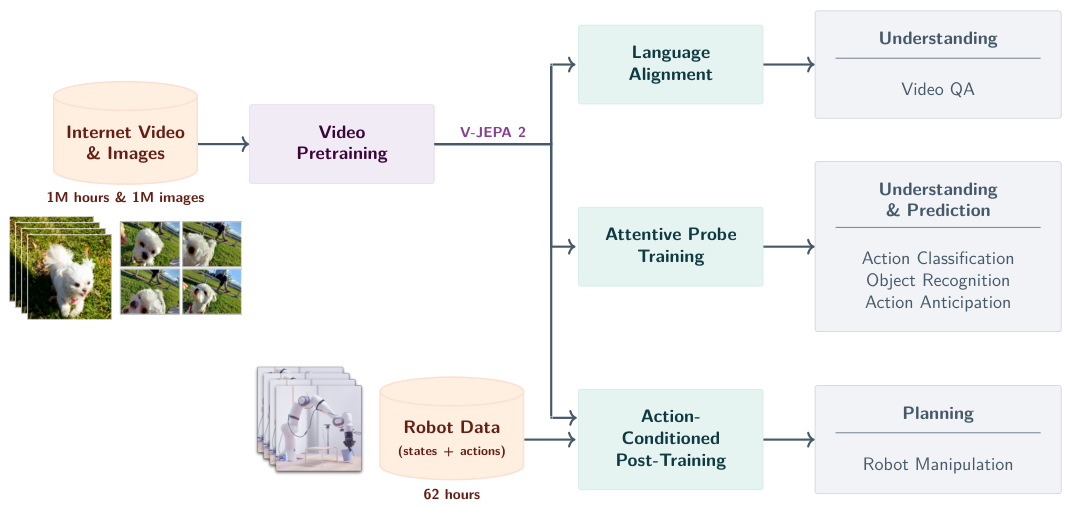
\includegraphics[width=0.9\linewidth,height=0.9\textheight,keepaspectratio]{assets/New-Lecture_JEPA_models/vjepa2_paper_fig1_overview.png}
      {\scriptsize Assran et al.\ (2025): overview of pre-training, alignment, and robotics post-training.}
  \end{columns}
\end{frame}

\begin{frame}{V-JEPA 2: End-to-End System Overview}
  \begin{columns}[T,onlytextwidth]
    \column{0.35\textwidth}
    {\footnotesize
    \begin{itemize}\itemsep0.26em
      \item[\textcolor{red}{$\blacktriangleright$}] Stage \textbf{A:} SSL on web video/images $\rightarrow$ strong motion and appearance understanding.
      \item[\textcolor{red}{$\blacktriangleright$}] Stage \textbf{B:} \textbf{language alignment}---project video tokens into an LLM with small attentive stacks so the backbone supports VQA and reasoning.
      \item[\textcolor{red}{$\blacktriangleright$}] Stage \textbf{C:} optional \textbf{action-conditioned} head (V-JEPA 2-AC) on tens of hours of robot data for latent planning.
    \end{itemize}
    }
    \column{0.65\textwidth}
    \centering
    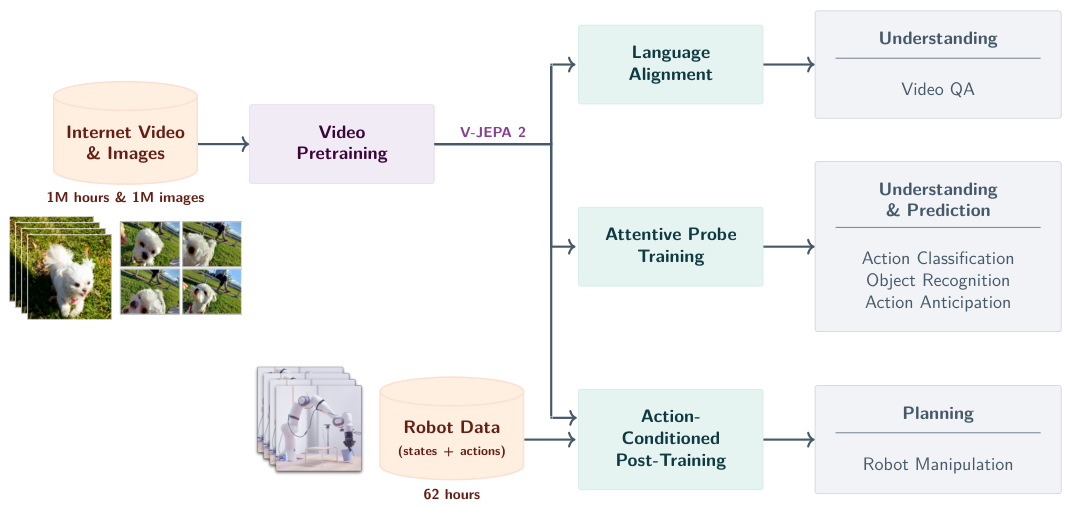
\includegraphics[width=0.9\linewidth,height=0.9\textheight,keepaspectratio]{assets/New-Lecture_JEPA_models/vjepa2_paper_fig1_overview.png}
    {\scriptsize Overview of pre-training, alignment, and robotics post-training.}
  \end{columns}
  \vspace{-0.1em}
  
\end{frame}

\begin{frame}{V-JEPA 2: Multi stage training}
  \centering
  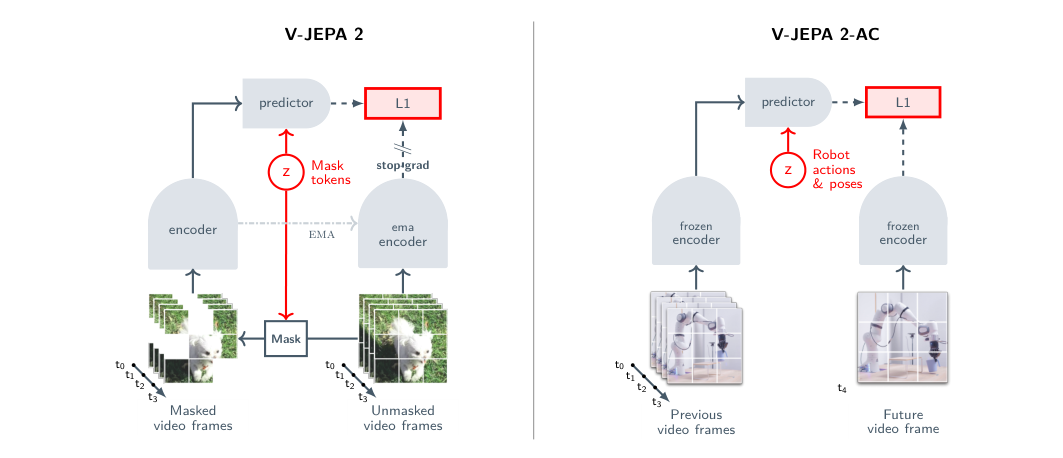
\includegraphics[width=0.9\linewidth,height=0.7\textheight,keepaspectratio]{assets/New-Lecture_JEPA_models/vjepa2_paper_fig2_multistage.png}
  \break
  {\scriptsize Assran et al.\ (2025): multistage training.} 
  {\footnotesize
  \begin{itemize}
    \item \textbf{V-JEPA 2:}
    \begin{itemize}   
      \item Video clips divided into tokens; a subset is masked.
      \item Encoder processes masked sequence to produce token embeddings.
      \item Mask tokens concatenated with encoder outputs.
      \item Predictor regresses to targets computed by an EMA encoder using $L_1$ loss.
    \end{itemize}
  \end{itemize}
  }
\end{frame}

\begin{frame}{V-JEPA 2: Multi stage training}
  \centering
  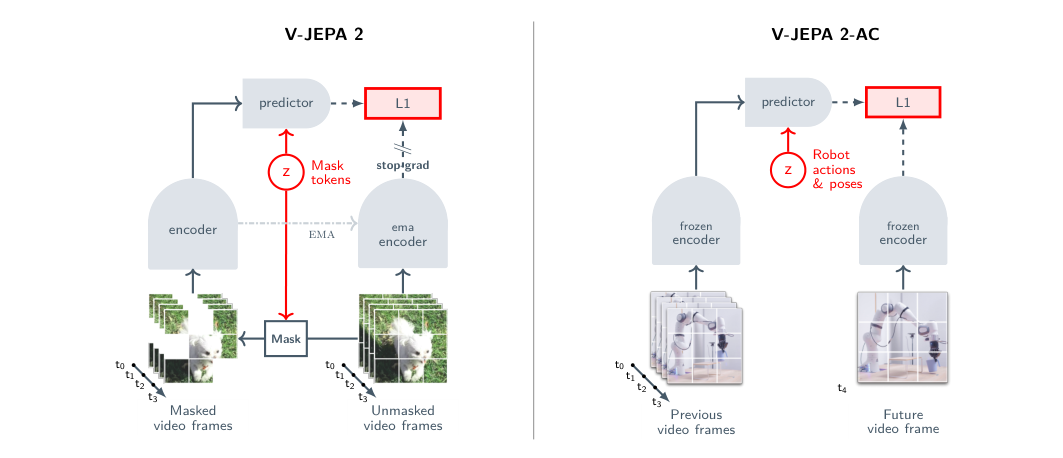
\includegraphics[width=0.9\linewidth,height=0.7\textheight,keepaspectratio]{assets/New-Lecture_JEPA_models/vjepa2_paper_fig2_multistage.png}
  \break
  {\scriptsize Assran et al.\ (2025): multistage training.} 
  {\footnotesize
  \begin{itemize}
    \item \textbf{V-JEPA 2-AC:}
    \begin{itemize}
      \item Freeze pretrained encoder and train action-conditioned predictor on top.
      \item Use autoregressive prediction to model future frame representations based on past frames, actions, and end-effector states.
    \end{itemize}
  \end{itemize}
  }
\end{frame}

\begin{frame}{V-JEPA 2: Performance}
  \centering
  \vspace{0.3em}
  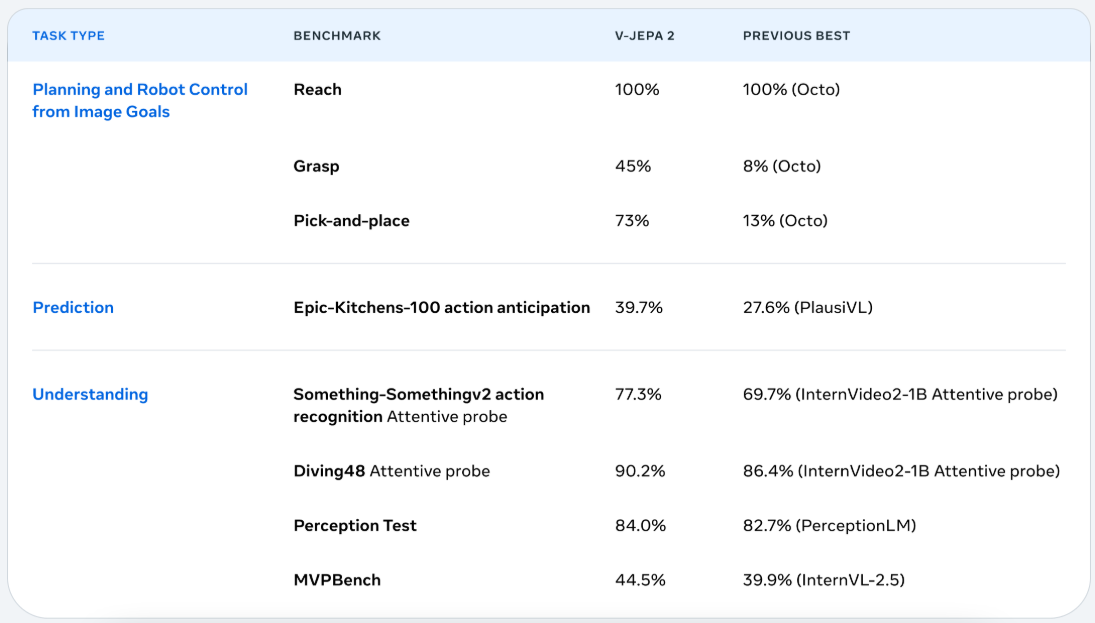
\includegraphics[width=0.9\linewidth,height=0.7\textheight,keepaspectratio]{assets/New-Lecture_JEPA_models/vjepa2_paper_fig3_performance.png}
  \linebreak
  {\scriptsize Assran et al.\ (2025): performance; see also \href{https://ai.meta.com/research/vjepa/}{Meta AI V-JEPA blog post}.}
\end{frame}

% \begin{frame}{V-JEPA 2: Performance}
%   \begin{itemize}\itemsep0.28em
%     \item[\textcolor{red}{$\blacktriangleright$}] \textbf{Fine-grained motion:} Something-Something v2 top-1 \textbf{77.3} (paper-reported).
%     \item[\textcolor{red}{$\blacktriangleright$}] \textbf{Action anticipation:} Epic-Kitchens-100 recall@5 \textbf{39.7}, described as strong vs.\ prior task-specialized models.
%     \item[\textcolor{red}{$\blacktriangleright$}] \textbf{Video QA (after LLM alignment):} e.g.\ PerceptionTest \textbf{84.0}, TempCompass \textbf{76.9} at an \textbf{8B-parameter} coupled stack (paper-reported).
%     \item[\textcolor{red}{$\blacktriangleright$}] \textbf{Robotics:} V-JEPA 2-AC trained on \textbf{$<$62 hours} of Droid-style trajectories; \textbf{zero-shot} Franka pick--place demos in \textbf{unseen labs} without environment-specific teleoperation or task rewards (as claimed in the paper abstract).
%   \end{itemize}
%   {\scriptsize Treat numbers as \textbf{snapshot} results from Assran et al.; see \href{https://arxiv.org/pdf/2506.09985}{PDF} for protocols and ablations.}
% \end{frame}
